\documentclass[aspectratio=169]{beamer}

\usetheme{Warsaw}
\usecolortheme{default}

\usepackage[T1]{fontenc}
\usepackage{lmodern}
\usepackage{graphicx}
\usepackage{adjustbox}
\usepackage{booktabs}
\usepackage{xcolor}

\definecolor{PUT-blue}{RGB}{0,84,147}
\definecolor{PUT-dark}{RGB}{0,45,85}
\definecolor{highlight}{RGB}{230,126,34}
\definecolor{commentbg}{RGB}{245,248,252}

\setbeamercolor{palette primary}{bg=PUT-blue,fg=white}
\setbeamercolor{palette secondary}{bg=PUT-dark,fg=white}
\setbeamercolor{palette tertiary}{bg=PUT-blue,fg=white}
\setbeamercolor{structure}{fg=PUT-blue}
\setbeamercolor{block body}{bg=commentbg}
\setbeamertemplate{headline}{}
\setbeamertemplate{footline}{%
  \leavevmode%
  \hbox{%
    \begin{beamercolorbox}[
      wd=.40\paperwidth,
      ht=2.75ex,
      dp=1.125ex,
      left,
      leftskip=.4cm,
      rightskip=.3cm
    ]{author in head/foot}%
      \usebeamerfont{author in head/foot}\insertshortauthor%
    \end{beamercolorbox}%
    \begin{beamercolorbox}[
      wd=.48\paperwidth,
      ht=2.75ex,
      dp=1.125ex,
      left,
      leftskip=.3cm,
      rightskip=.15cm
    ]{title in head/foot}%
      \usebeamerfont{title in head/foot}\insertshorttitle%
    \end{beamercolorbox}%
    \begin{beamercolorbox}[
      wd=.12\paperwidth,
      ht=2.75ex,
      dp=1.125ex,
      right,
      leftskip=.15cm,
      rightskip=.4cm
    ]{title in head/foot}%
      \usebeamerfont{title in head/foot}\insertframenumber/\inserttotalframenumber%
    \end{beamercolorbox}%
  }%
}

\graphicspath{{../notebooks/plots/}{../notebooks/plots/results/}}

% Bottom detail line under figures (one idea per slide).
\newcommand{\slidecomment}[1]{%
  \vspace{0.3em}
  \begin{beamercolorbox}[wd=\linewidth,rounded=true,sep=0.7ex]{block body}
    \small #1
  \end{beamercolorbox}
}

\newcommand{\slidefigure}[2][]{%
  \begin{center}
  \adjustbox{max width=\linewidth, max height=0.50\textheight, keepaspectratio, center, #1}{%
    \includegraphics{#2}%
  }%
  \end{center}
}

\newcommand{\slidefigureshort}[2][]{%
  \begin{center}
  \adjustbox{max width=\linewidth, max height=0.42\textheight, keepaspectratio, center, #1}{%
    \includegraphics{#2}%
  }%
  \end{center}
}

% Two wide figures on one slide (shared vertical budget).
\newcommand{\slidefigurepair}[2]{%
  \vspace{-0.35em}
  \begin{center}
  \adjustbox{max width=\linewidth, max height=0.24\textheight, keepaspectratio, center}{%
    \includegraphics{#1}}%
  \par\vspace{0.12em}
  \adjustbox{max width=\linewidth, max height=0.22\textheight, keepaspectratio, center}{%
    \includegraphics{#2}}%
  \end{center}
}

\newcommand{\slidestrip}[2][]{%
  \adjustbox{width=\linewidth, center, #1}{\includegraphics{#2}}%
}

\newcommand{\timingnote}[1]{\note{#1}}

\title{Generative Models for Cat Face Synthesis}
\subtitle{Which architecture wins on the same $128 \times 128$ cat faces?}
\author{Paweł Pozorski \and Paweł Florek}
\institute{Warsaw University of Technology}
\date{\today}

\begin{document}

\begin{frame}[plain]
  \titlepage
\end{frame}

\section{Setup}

\begin{frame}{From Raw Photos to a Fair Benchmark}
  \framesubtitle{Landmark crop fixes varying resolution; every model sees the same tensors}
  \begin{columns}[T]
    \begin{column}{0.54\linewidth}
      \small
      \begin{itemize}
        \item \textbf{Crop:} \texttt{.cat} landmarks $\rightarrow$ face box, $128 \times 128$.
        \item \textbf{Split:} $90/10$ train/val; normalize to $[-1,1]$.
        \item \textbf{Budget:} Apple MPS, early stopping, $138$ cat-face runs.
        \item \textbf{Score:} FID on $N{=}1000$ samples; three seeds per grid cell.
      \end{itemize}
    \end{column}
    \begin{column}{0.44\linewidth}
      \adjustbox{width=\linewidth, center}{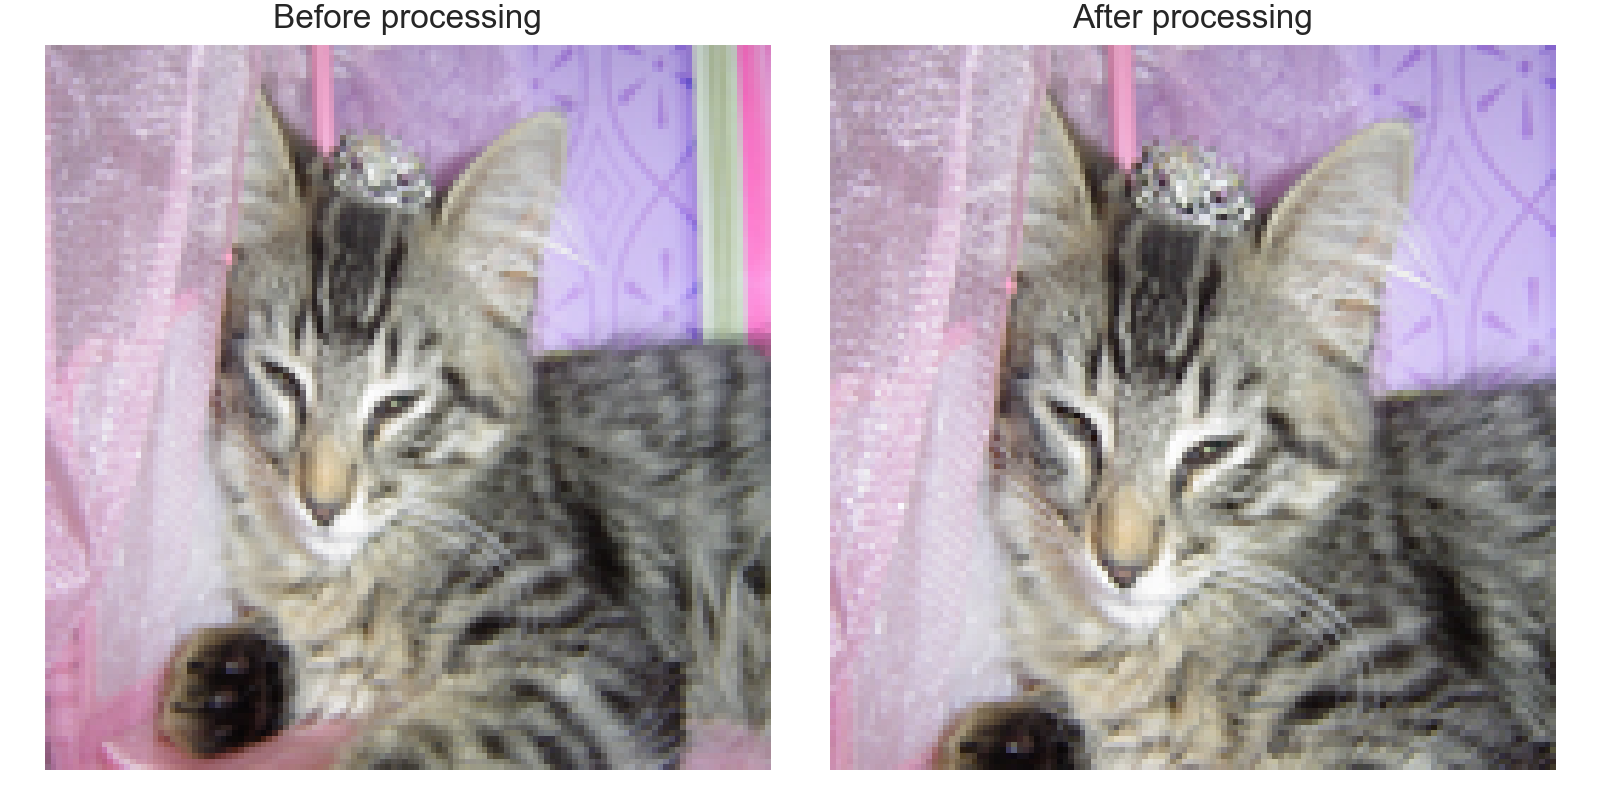
\includegraphics{preprocessing_comparison.png}}
    \end{column}
  \end{columns}
  \timingnote{75\,s. ``We removed resolution noise before comparing architectures.''}
\end{frame}

\begin{frame}{Seven Generators, One Protocol}
  \framesubtitle{Same optimizer family, logging, and evaluation scripts for all}
  \small
  \begin{tabular}{@{}ll@{}}
    \toprule
    \textbf{Family} & \textbf{Models in the sweep} \\
    \midrule
    VAE & $\beta$-VAE, VQ-VAE-1 \\
    GAN & WGAN-GP, SN-GAN \\
    Diffusion & DDIM (pixels), Tiny LDM (VQ latents) \\
    VQ prior & PixelCNN (+ fixed Tiny LDM for timing) \\
    \bottomrule
  \end{tabular}
  \vspace{0.5em}

  Grid: $44$ hyperparameter cells $\times$ 3 seeds. GANs use stabilization (GP / spectral norm) to limit mode collapse.
  \timingnote{75\,s. Point at the table; one line per family, then move on.}
\end{frame}

\section{Rankings}

\begin{frame}{FID Leaderboard}
  \framesubtitle{Stabilized GANs beat VAEs and VQ-prior baselines}
  \slidefigure{fid_best_runs.png}
  \slidecomment{\textbf{Headline:} WGAN-GP $174.4$, SN-GAN $226.1$. VAEs and PixelCNN trail above $240$. DDIM/Tiny LDM trained but missing from the FID export.}
  \timingnote{75\,s. Pause on the gap between GAN and VAE bars.}
\end{frame}

\begin{frame}{Hyperparameters Move the Needle}
  \framesubtitle{Best vs.\ worst grid cell can differ by $>110$ FID points}
  \slidefigure{fid_grid_distribution.png}
  \slidecomment{\textbf{Winners:} batch $128$, symmetric learning rates, $n_{\text{critic}}{=}5$ (WGAN-GP). SN-GAN: turn off hflip aug.\ on the best cell.}
  \timingnote{60\,s. ``Tuning matters as much as picking the family.''}
\end{frame}

\section{Look Closer}

\begin{frame}{Do the Samples Match the Scores?}
  \framesubtitle{Sharp GAN faces; soft VAEs; diverse poses on cat-only data}
  \slidefigureshort{samples_best_per_family.png}
  \slidecomment{\textbf{Mode collapse:} not obvious on WGAN-GP/SN-GAN boards---varied colors and poses. Next slide zooms into GAN vs.\ VAE; diffusion families sit between on the full grid.}
  \timingnote{60\,s. Orient the audience across all seven families; save the GAN--VAE contrast for the next slide.}
\end{frame}

\begin{frame}{GAN vs.\ VAE Head-to-Head}
  \framesubtitle{Best checkpoint per family: FID $174.4$ vs.\ $278.3$}
  \slidefigure{samples_gan_vs_vae.png}
  \slidecomment{\textbf{Gap:} WGAN-GP keeps whiskers, eyes, and fur texture. $\beta$-VAE captures pose and color but blurs fine structure---the usual VAE trade-off.}
  \timingnote{45\,s. Left grid, then right; let the visual difference land before speaking.}
\end{frame}

\begin{frame}{Latent Space: Smooth or Sharp?}
  \framesubtitle{Ten frames per model: $z_1 \rightarrow z_2$ with eight linear steps}
  \vspace{-0.35em}
  {\scriptsize $\beta$-VAE \hfill seed~3407\par}
  \vspace{0.1em}
  \slidestrip{interpolation_beta_vae_seed3407.png}
  \vspace{0.35em}
  {\scriptsize WGAN-GP \hfill seed~3407\par}
  \vspace{0.1em}
  \slidestrip{interpolation_wgan_gp_seed3407.png}
  \slidecomment{\textbf{Takeaway:} interpolation is meaningful in both models---faces morph, not noise---but WGAN-GP keeps detail; $\beta$-VAE stays soft throughout.}
  \timingnote{60\,s. Trace one morph left-to-right with your cursor.}
\end{frame}

\begin{frame}{Speed vs.\ Autoregression on VQ Codes}
  \framesubtitle{Same decoder; different prior}
  \vspace{-0.2em}
  \begin{center}
  \adjustbox{width=0.98\linewidth, center}{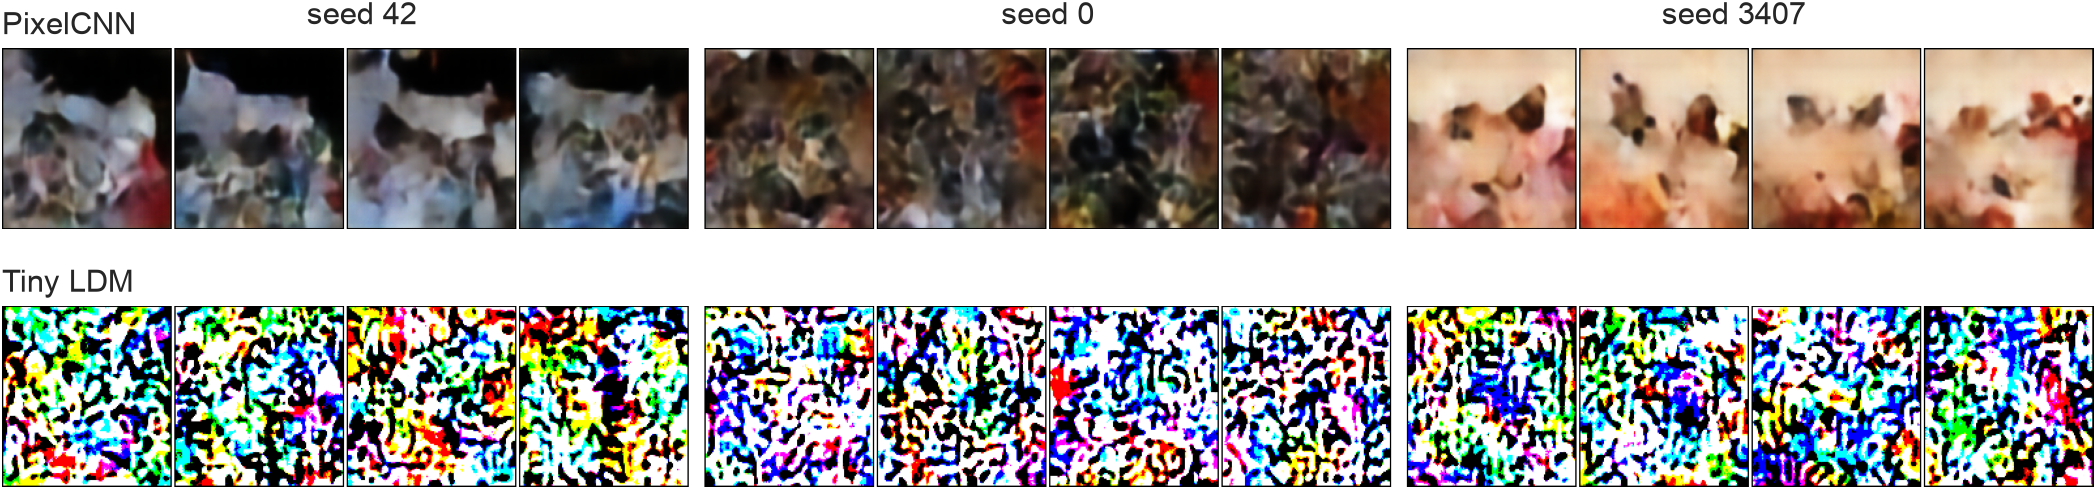
\includegraphics{prior_samples_panel.png}}%
  \end{center}
  \slidecomment{\textbf{Trade-off:} Tiny LDM samples $\sim$5$\times$ faster ($0.050$ vs.\ $0.260$\,s/image on MPS), but these checkpoints decode to unstructured noise. PixelCNN is slower yet retains weak coarse blobs---neither is a usable cat prior here.}
  \timingnote{45\,s. Lead with the speed numbers, then the visual failure of Tiny LDM.}
\end{frame}

\begin{frame}{What Happens on Dogs + Cats?}
  \framesubtitle{Chimera extension: unconditional WGAN-GP at $64 \times 64$}
  \slidefigurepair{chimera_panel.png}{chimera_progress_chimera_64_seed0.png}
  \vspace{-0.1em}
  \slidecomment{\textbf{Contrast:} cat-only WGAN-GP $\rightarrow$ clean faces (sample slides). Mixed data $\rightarrow$ hybrids, not separate dog and cat modes.}
  \timingnote{60\,s. Top: three seeds; bottom: training progression for seed~0.}
\end{frame}

\section{Close}

\begin{frame}{Three Lessons}
  \begin{enumerate}
    \item \textbf{Pick WGAN-GP or SN-GAN for sharp cat faces} --- best FID, stable training, diverse samples.
    \item \textbf{VAEs and VQ priors trade quality for structure or speed} --- blur, higher FID, or slower autoregression.
    \item \textbf{Unconditional models average mixed classes} --- chimera faces blend species; do not expect clean separation.
  \end{enumerate}
  \vspace{0.4em}
  {\small Limits: partial FID seed coverage, diffusion FIDs not exported, one saved interpolation seed.}
  \timingnote{60\,s. End on lesson 3---it connects back to the opening question.}
\end{frame}

\begin{frame}[plain]
  \centering
  \Huge \textbf{Thank You}
  \vspace{1.2em}

  \normalsize
  Paweł Pozorski, Paweł Florek \\
  Warsaw University of Technology \\
  {\small \{pawel.pozorski, pawel.florek\}.stud@pw.edu.pl}
  \vspace{1em}
  {\small Report and code: \texttt{github.com/FlorekPawel/gen-cats}}
\end{frame}

\end{document}
